\documentclass[10pt]{article}
\usepackage[T1]{fontenc}
\usepackage[utf8]{inputenc}
\usepackage{lmodern}
\usepackage[a4paper,margin=24mm]{geometry}
\usepackage{amsmath,amssymb,booktabs,graphicx,array}
\usepackage{xcolor}
\definecolor{flm}{HTML}{A74C20}
\usepackage[colorlinks=true,linkcolor=flm,citecolor=flm,urlcolor=flm]{hyperref}
\usepackage{microtype}
\setlength{\parskip}{5pt}
\setlength{\parindent}{0pt}
\setlength{\emergencystretch}{2em}
\renewcommand{\arraystretch}{1.15}
\graphicspath{{figures/}}
\newcommand{\code}[1]{\texttt{\detokenize{#1}}}

\newcommand{\ChoiceRows}{%
BPTT & 100.00 & 100.00 & 100.00 & 100.0--100.0 \\
Fixed core & 100.00 & 99.74 & 86.46 & 74.2--100.0 \\
Eligibility & 100.00 & 85.29 & 83.33 & 50.0--100.0 \\
No trace history & 88.28 & 66.67 & 50.00 & 50.0--50.0 \\
Reward + eligibility & 83.33 & 83.33 & 50.00 & 50.0--50.0 \\
}

\hypersetup{pdftitle={FLM: Forward Eligibility, Reversal Learning and Physical Choice},pdfauthor={Kuber},pdflang={en}}
\title{\textbf{FLM: Forward Eligibility and Learned Choice}\\[6pt]\large A controlled learning-rule comparison and physical action assay}
\author{Kuber\\\href{https://flm.kuber.studio}{flm.kuber.studio}}
\date{10 September 2026 --- working research note}
\begin{document}
\maketitle
\begin{abstract}
We compare full backpropagation through time, fixed-core readout learning, local forward eligibility, a no-history control, and reward-modulated eligibility in a 256-neuron fly-wired rate network. Fifteen fixed-budget runs learn, reverse and restore a delayed cue association. All methods receive identical stimuli and initialization within each of three seeds. At the final 48-frame delay probe, mean accuracy is 100\% for backpropagation, 86.46\% for the fixed-core control, 83.33\% for supervised eligibility, and 50\% for both no-history and reward eligibility. Thus this experiment provides no local-learning advantage over backpropagation. A separate 40-case MuJoCo assay verifies that recorded learned choices drive physical turns through a designed gait controller. These results establish a reproducible learning-and-action interface, with substantial limitations; they do not establish language-to-motor transfer or biological validity.
\end{abstract}

\section{Relation to the language model}
This study is separate from FLM's 600k-parameter WikiText and BabyLM language experiments. It reuses the fast/slow rate recurrence and anatomy-only selection procedure, with a four-channel sensory input and a two-action output. The graph contains 256 central intrinsic neurons, 6,678 directed edges and 32 readout pools. Its source is the same verified MaleCNS representation \cite{malecns}, but it is a different induced subset from the 1,024-neuron language core. Input channels and action projections are engineered; no sensory or descending biological pathway is claimed.

Eligibility-based learning is established prior work, applicable beyond fly wiring. The e-prop framework motivates a factorization into forward eligibility and neuron-specific learning signals \cite{bellec}. Here we derive a local temporal approximation for FLM's particular normalized rate dynamics. The model has no spikes, synaptic delays or biophysical units, and is not a reproduction of e-prop's spiking experiments.

\section{Dynamics and direct derivatives}
For edge $j\to i$, let $v_{ij}=b_{ij}\exp(\theta_{ij})$ and
$W_{ij}=v_{ij}/\sum_k|v_{ik}|$, where $b_{ij}$ carries the retained contact-derived
magnitude and assumed presynaptic sign. Edge logits are projected to $[-3,3]$
after updates. With $q_i=\sum_j W_{ij}h_j^{\mathrm{prev}}$, the network uses
\begin{align}
z_i &= \tanh(A_i x+b_i+gq_i),\\
h_i &= (1-\alpha_i)h_i^{\mathrm{prev}}+\alpha_i z_i,\\
s_i &= (1-\beta_i)s_i^{\mathrm{prev}}+\beta_i h_i.
\end{align}
The existing sigmoid bounds give $\alpha\in(.05,.95)$, $\beta\in(.002,.100)$,
and $g\in(.05,3)$. The normalized edge's direct derivative is
\begin{equation}
\frac{\partial q_i}{\partial\theta_{ij}}
=W_{ij}h_j^{\mathrm{prev}}-|W_{ij}|q_i.
\end{equation}
Ignoring the second term would change the learning rule: incoming normalization
couples the effects of all weights arriving at the same postsynaptic neuron.

\newpage
\section{Forward credit and controls}
Define the local fast-state Jacobian
$J_i=1-\alpha_i+\alpha_i(1-z_i^2)gW_{ii}$. For a parameter associated with
neuron $i$, retain fast and slow traces:
\begin{align}
e_{h,i} &\leftarrow J_i e_{h,i}^{\mathrm{prev}}+d_{h,i},\\
e_{s,i} &\leftarrow (1-\beta_i)e_{s,i}^{\mathrm{prev}}+\beta_i e_{h,i}+d_{\beta,i}.
\end{align}
Direct input derivatives use $\alpha_i(1-z_i^2)x$; bias replaces $x$ with one.
Edge derivatives multiply equation (4) by $\alpha_i(1-z_i^2)g$. Alpha and gain
logits use their direct sigmoid derivatives. Beta contributes
$d_{\beta,i}=(h_i-s_i^{\mathrm{prev}})\partial\beta_i/\partial\mathrm{logit}$.
The complete expressions and implementation are in the declared protocol.

At the final decision, instantaneous derivatives through pooling, LayerNorm and
the readout supply $L_h,L_s$. Core updates use $\sum_{\mathrm{batch}}(L_he_h+L_se_s)$;
the shared gain also sums over neurons. Earlier states have no autograd history
in the forward conditions. This approximation drops temporal credit carried
through other neurons. Tests match full autograd when those routes are absent,
verify the normalized direct derivative by finite differences, and check exact
state parity between the ordinary and eligibility paths. They do not prove
equality with the full recurrent gradient.

All conditions use SGD at .03, batch eight, no momentum or weight decay, and
global gradient clipping at one. The fixed-core control trains only 258 output
and normalization parameters. The other conditions may train all 8,729 parameters.
The no-history control clears trace history each frame. The reward condition
samples an action and uses $-(r-\bar r)\log p(a)$, with $r\in\{0,1\}$ and the
previous exponential reward baseline (decay .95, initially .5). Its separate
action RNG preserves the shared sensory stream. Binary correctness also reveals
whether the other action would succeed, so this task does not demonstrate
learning from strictly less target information.

\section{Registered task and final measurements}
Two cue frames precede an integer delay sampled uniformly from 4--12 and one
query frame. An independent Gaussian distractor (SD .2) is present throughout.
Each balanced batch contains four examples of each cue. The original association
is trained for 300 updates, its reverse for 300, then the original for 300:
7,200 episodes per run. Seeds are 17, 29 and 41. State and traces reset each
episode; weights persist. No phase flag is supplied.

Every 100 updates and initially, fixed panels contain 256 balanced episodes per
delay (4, 8, 12, 24, 48). Panels are repeatedly inspected diagnostics, not an
untouched test set or a checkpoint-selection criterion. Table 1 reports the
restored rule after the fixed 900 updates. The two association scores are
mutually exclusive, not independent tasks.

\begin{table}[h]\centering\small
\caption{Final accuracy (\%). Means over three seeds; the last column is the
observed seed range at delay 48, not a confidence interval.}
\begin{tabular}{lrrrr}\toprule
Learning rule & Delay 8 & Delay 12 & Delay 48 & Range, 48\\\midrule
\ChoiceRows
\bottomrule\end{tabular}
\end{table}

\newpage
\section{Reversal and retention}
\begin{figure}[!ht]\centering
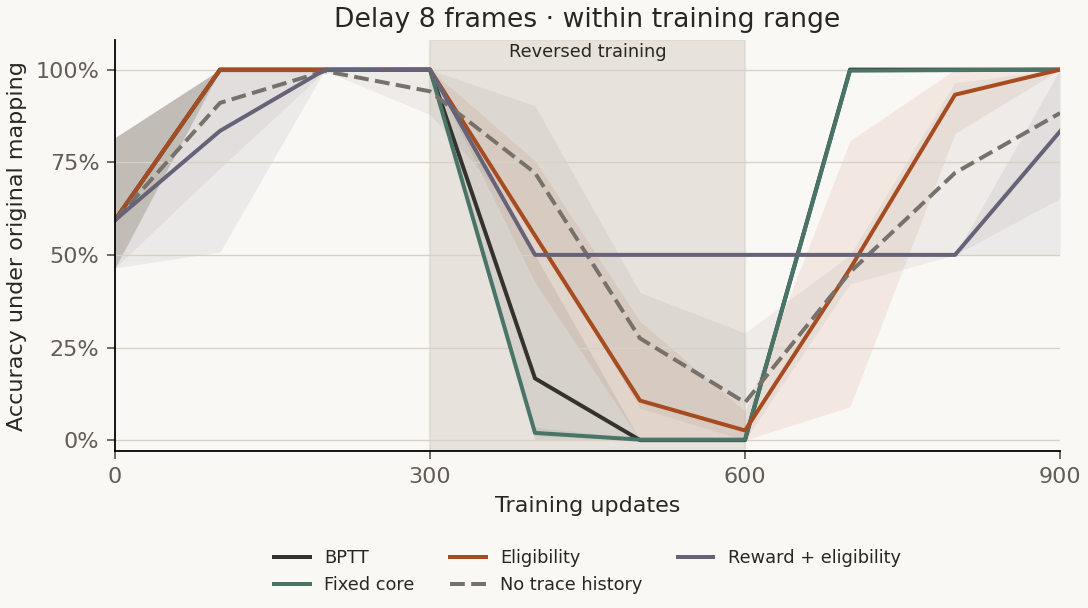
\includegraphics[width=.89\linewidth]{choice-reversal-delay8.png}
\caption{Within-range delay. The vertical axis always scores the original
association; descending during reversed training therefore indicates learning
the new rule. Curves average three seeds; bands span their observed range.}
\vspace{4mm}
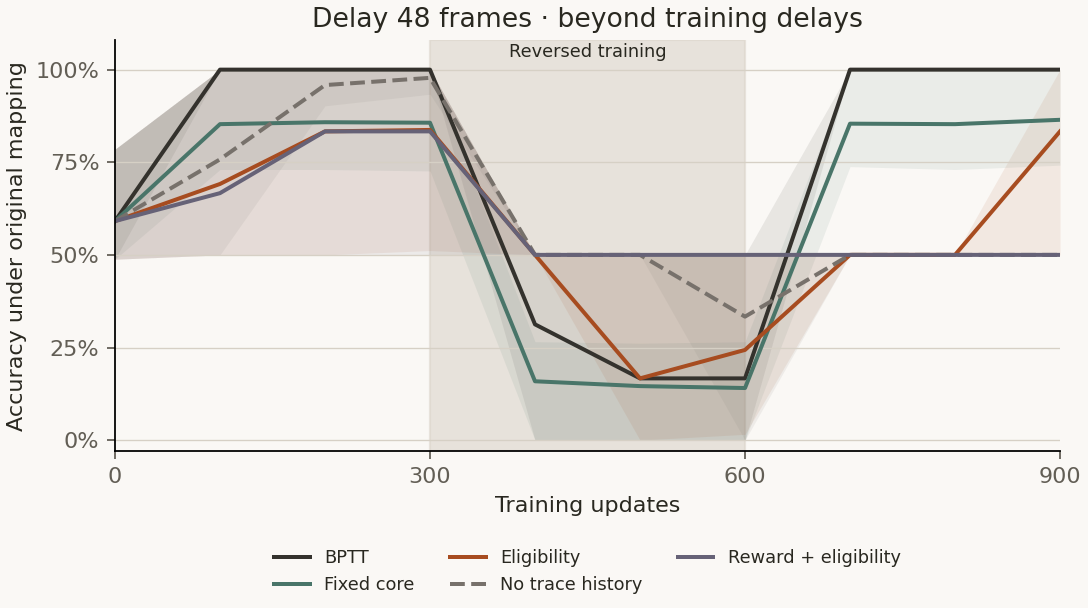
\includegraphics[width=.89\linewidth]{choice-reversal-delay48.png}
\caption{Delay extrapolation. Backpropagation finishes at 100\% in all three
seeds. Supervised eligibility finishes at 50\%, 100\%, 100\%; the fixed core
finishes at 100\%, 85.16\%, 74.22\%. No-history and reward eligibility finish
at 50\% in every seed. This narrow task does not establish a general ranking.}
\end{figure}

\clearpage
\section{From a learned choice to a physical turn}
The predeclared physical assay uses seed 17, checkpoints 0/300/600/900 and both
zero-distractor cues at delay eight, for each of the five learning conditions.
Argmax action zero selects descending command $[.4,1.2]$; action one selects
$[1.2,.4]$. Each case starts independently from the same body pose and controller
seed, and runs one simulated second (10,000 physics steps) using FlyGym 2.1.0,
MuJoCo 3.9.0 and its designed hybrid turning controller \cite{neuromechfly}.

The complete assay contains 40 separately simulated cases and 2 unique descending commands. The measured heading sign matches the chosen command in all 40 cases. Neural choices agree with the rule associated with their checkpoint in 33 of 40 cases, including the untrained controls. All recorded generalized positions are exactly equal between cases with the same command and initialization. This confirms deterministic action execution, not independent motor skills or a statistical motor-learning benchmark.


The two commands change heading by approximately $+2.811$ and $-2.556$ radians,
respectively. Training changes cue-dependent action probabilities and can change
the resulting trajectory. The published archive binds each neural decision and
state to its checkpoint and physical trajectory. The video shows the predeclared
supervised-eligibility, update-300, cue-zero case.

The neural decision is recorded before the physics replay. FLM does not receive
online proprioception, train joint trajectories, learn balance or adapt from a
physical reward in this assay. The gait and contact controller supply those
motor functions. The female NeuroMechFly body accompanies a male-connectome
subset. These limits are distinct from the browser body's illustrative pose and
from any future transfer of language-trained state into motor decisions.

\section{What the experiment changes}
The implemented forward rule is executable and can learn a cue association, but
it is not a demonstrated improvement over full backpropagation. The fixed-core
control's strength exposes a limitation of the task: accessible state already
contains much of the required information. Reversal and long-delay failures
show sensitivity to plasticity and initialization, not proof of a biological
mechanism. Anatomical advantage needs a matched rewired graph; useful learned
memory needs tasks that a fixed readout cannot readily solve.

Eligibility storage is 558,464 tensor bytes for batch eight, plus 16,384 recurrent
state bytes. It is fixed with episode length but grows with parameter count.
This is not a measured peak-memory, runtime or energy advantage over BPTT.
The output normalization and feedback routes are engineered and nonlocal.
Next comparisons should isolate plasticity sites, inspect gradient alignment,
strengthen the memory task and add sensory feedback. Language transfer and
scaling remain unfinished experiments.

\section{Reproduction and artifacts}
Run \code{python -m flm.behavior_study}, then
\code{python -m flm.behavior_report}. Use the isolated embodied environment for
\code{python experiments/embodiment/learned_choice.py --video}, followed by
\code{python scripts/physical_choice_report.py}. Source revisions, stimulus stream
hashes, every panel prediction, failed cases and neural states are retained.
The website publishes JSON, CSV, plotted data and trajectory archives.
The implementation and larger program are available at
\url{https://github.com/Kuberwastaken/flm} and
\url{https://flm.kuber.studio/#research}.

\bibliographystyle{plain}\bibliography{references}
\end{document}
